\documentclass[a4paper,11pt]{article}
\usepackage[scale=0.85]{geometry}
\usepackage{titling}
\usepackage{amsmath,amsfonts}
\usepackage{xcolor}
\usepackage{braket}
\usepackage{bm}
\usepackage{tensor}
\usepackage{cleveref}
% \usepackage{MnSymbol}
\usepackage{mhchem}
\usepackage{graphicx}
\usepackage{cite}
\usepackage{booktabs}
\usepackage{wrapfig}
\usepackage{bbm}
\usepackage{framed}
\usepackage{frame}
\usepackage[shortlabels]{enumitem}
\title{Homework for Week 11-13}
\author{Chen Xue  2022311901}
\begin{document}
\maketitle

\section{Hamiltonian Formulation of electrodynamics in Continuum}
\paragraph{a)}
\begin{equation} \label{Lagrangian}
    \mathcal{L} 
    = \sum_i \frac{\epsilon_0}{2e^2} f_{i0}^2 
    - \sum_{i<j} \frac{1}{2\mu_0 e^2} f_{ij}^2
    + \sum_{\mu} a_{\mu}J^{\mu},
    \hspace*{1em}
    f_{\mu \nu} \equiv \partial_{\mu}a_{\nu} - \partial_{\nu} a_{\mu}
\end{equation}
The Lagrangian equation is
\begin{equation} \label{Leq}
    \frac{\partial \mathcal{L}}{\partial a_{\mu}}
    = \partial_t \frac{\partial \mathcal{L}}{\partial \partial_t a_{\mu}}
    + \partial_{i} \frac{\partial \mathcal{L}}{\partial \partial_{i}a_{\mu}}
\end{equation}
for $a_0$, inserting (\ref{Lagrangian}) into (\ref{Leq}) we get 
\begin{equation} \label{J^0}
    J^0 
    = \frac{\epsilon_0}{e^2} \nabla \cdot \bm{f_0} 
    = \frac{\epsilon_0}{e^2} (\nabla^2 a_0 - \partial_t \nabla \cdot \bm{a})
\end{equation}
where $ \bm{f_0} \equiv (f_{10}, \dots, f_{d0}) = \nabla a_0 - \partial_t \bm{a}$. This is \textbf{Gauss's law} if we integrate $\bm{f_0}$ as electric field. In the same way, we can get the following equations
\begin{equation}
    J^k 
    = -\frac{\epsilon_0}{e^2} \left( \partial_t \partial_k a_0 - \partial_t^2 a_k\right)
    + \frac{1}{\mu_0 e^2} \left(\partial_k (\nabla \cdot \bm{a}) - \nabla^2 a_k\right)
\end{equation}
which can be written as
\begin{equation}
    \bm{J} 
    = -\frac{\epsilon_0}{e^2}(\partial_t \nabla a_0 - \partial_t^2 \bm{a})
    + \frac{1}{\mu_0 e^2} (\nabla(\nabla \cdot \bm{a}) - \nabla^2 \bm{a})
    = -\frac{\epsilon_0}{e^2} \partial_t \bm{f_0} 
    + \frac{1}{\mu_0 e^2} \nabla \times (\nabla \times \bm{a})
\end{equation}
This can be viewed as \textbf{Amp\`ere's circuital law with Maxwell's addition} by interpreting $\nabla \times \bm{a}$ as magnetic field. This also give \textbf{Gauss's law for magnetism} $\nabla \cdot (\nabla \times \bm{a}) = 0$. Also, $\nabla \times (\nabla a_0 - \partial _t \bm{a}) = -\partial_t (\nabla \times \bm{a})$, which is \textbf{Maxwell-Faraday equation}.
The above factors can be changed to the usual ones by $ \frac{\epsilon_0}{e^2} \rightarrow \epsilon_0, \mu_0 e^2 \rightarrow \mu_0$. In the above take $e$ as an intrinsic property of the EM field.

\paragraph{b)}
Perform Hubbard-Stratonovich transformation s.t. $f_{i0}^2 \rightarrow -\pi_i^2$ as following
\begin{equation}
    \mathcal{L'} 
    = -\sum_{i} \frac{e^2}{2\epsilon_0}\pi_i^2 
    - \sum_{i<j} \frac{1}{2\mu_0 e^2} f_{ij}^2
    + \sum_{\mu} a_{\mu}J^{\mu}
    - \sum_i f_{i0}\pi_i
\end{equation}
integrate out $a_0$ by part integration, we get $ J^0 - \nabla \cdot \bm{\pi} = 0$ (\textcolor{red}{sign}). Also, 
\begin{equation}
    \mathcal{L'} = 
    - \sum_{i} \frac{e^2}{2\epsilon_0}\pi_i^2 
    - \sum_{i<j} \frac{1}{2\mu_0 e^2} f_{ij}^2
    + \sum_{i} a_{i}J^{i}
    + \sum_{i}(\partial_t a_i)\pi_i
\end{equation}
so the canonical conjugate of $a_i$ is $\pi_i$ as $\frac{\partial \mathcal{L'}}{\partial \partial_t a_i} = \pi_i$, and the Hamiltonian density is 
\begin{equation}
    \mathcal{H}
    = \sum_i \pi_i \partial_t a_i - \mathcal{L'}
    = \sum_{i} \frac{e^2}{2\epsilon_0}\pi_i^2 
    + \sum_{i<j} \frac{1}{2\mu_0 e^2} f_{ij}^2
    - \sum_{i} a_{i}J^{i}
\end{equation}
By Hamilton's equations of motion for the fields
\begin{equation}
    \frac{{\rm d}a_{i}}{{\rm d}t} = \frac{\delta \mathcal{H}}{\delta \pi_{i}},
    \hspace{3em}
    \frac{{\rm d}\pi_{i}}{{\rm d}t} = -\frac{\delta \mathcal{H}}{\delta a_{i}}
\end{equation}
where 
\begin{equation}
    \frac{\delta}{\delta a_{i}}
    = \frac{\partial}{\partial a_i} - \nabla \cdot \frac{\partial}{\partial (\nabla a_i)}
\end{equation}
then we get 
\begin{equation}
    \begin{aligned}
        &\frac{{\rm d} a_i}{{\rm d}t} = \frac{e^2}{\epsilon_0} \pi_i\\
        &\frac{{\rm d} \pi_i}{{\rm d} t} 
        = - J^i + \frac{1}{\mu_0 e^2}  \left(\partial_i (\nabla \cdot \bm{a}) - \nabla^2 a_i\right)
        = - J^i + \frac{1}{\mu_0 e^2}  \left(\nabla \times (\nabla \times \bm{a})\right)_i
    \end{aligned}
\end{equation}
together with $J^0 = \nabla \cdot \bm{\pi}$, we can view $\bm{\pi}$ as the electric field, $\nabla \times \bm{a}$ as the magnetic field. Then the Maxwell equations are naturally obtained. Compared these with \textbf{a)}, we can see that $\bm{\pi} = - \frac{\epsilon_0}{e^2}\bm{f_0}$.

\paragraph{c)}
Commutation relations are as follows
\begin{equation}
    [a_i(\bm{r},t), \pi_j (\bm{r'},t)] = i\hbar \delta(\bm{r} - \bm{r'})\delta_{ij}
\end{equation}
we want to calculate 
\begin{equation}
    [a_i, e^{-i \int {\rm d}^{\rm d}r \alpha \mathcal{G}}] 
    = -i e^{-i \int {\rm d}^{\rm d}r \alpha \mathcal{G}} 
    (\sum_j \int {\rm d}^{\rm d}r) \alpha(\bm{r})[a_i(\bm{r'},t), \mathcal{G}_j(\bm{r},t)]
\end{equation}
the summation and integral are calculated as
\begin{equation}
      (\sum_j \int {\rm d}^{\rm d}r)\alpha(\bm{r}) \frac{\partial}{\partial r_j}[a_i(\bm{r'},t), \pi_j(\bm{r},t)]
    = i\hbar  \int {\rm d}^{\rm d}r \alpha(\bm{r}) \frac{\partial}{\partial r_i} \delta(\bm{r} - \bm{r'})
    = -i\hbar \frac{\partial}{\partial r'_i} \alpha(\bm{r'})
\end{equation}
then we have
\begin{equation}
    e^{i \int {\rm d}^{\rm d}r \alpha \mathcal{G}} a_i e^{-i \int {\rm d}^{\rm d}r \alpha \mathcal{G}}
    = a_i - \hbar \partial_i \alpha
\end{equation}
so $\mathcal{G}$ is the gauge transformation generator.\\
The commutator between $\mathcal{G}$ and $H$ when $J^{\mu} =0$ is
\begin{equation}
      \int {\rm d}^d r [\mathcal{G}(r'), \mathcal{H}(r)]
    = \int {\rm d}^d r \sum_{ijk} \frac{1}{2\mu_0 e^2} 
    [ \frac{\partial}{\partial r'_i} \pi_i(r'),
      \frac{\partial}{\partial r_j} a_k(r) 
    - \frac{\partial}{\partial r_k}a_j(r)]f_{jk}(r) 
    = 0
\end{equation}
which means $\mathcal{G}$ represents a conservation. As $\mathcal{G} = J^0$, this means the conservation of particle number. When $J^{\mu} \neq 0$,
\begin{equation}
    \int {\rm d}^d r [\mathcal{G}(r'), \mathcal{H}(r)]
    = -\sum_{ij} \int {\rm d}^d r [\frac{\partial}{\partial r'_i} \pi_i(r'), a_j(r)]J^j(r)
    = i\hbar \sum_i \partial_i J^i
\end{equation}
recall that $ \mathcal{G} = J^0$, $\frac{{\rm d} J^0}{{\rm d}t} = \frac{1}{i\hbar}[J^0, H] = \nabla \cdot \bm{J}$, this is the current conservation equation.

\paragraph{d)}
Since 
\begin{equation}
    \hat{a_i}(r)\ket{\{a_i\}} = a_i(r)\ket{\{a_i\}}
\end{equation}
we can insert identity $ \mathbbm{1} = e^{i \int {\rm d}^{\rm d}r \alpha \mathcal{G}}  e^{-i \int {\rm d}^{\rm d}r \alpha \mathcal{G}}$ between operator and state, and multiply $e^{-i \int {\rm d}^{\rm d}r \alpha \mathcal{G}}$ from left to both sides. Then we get 
\begin{equation}
    (\hat{a_i} + \hbar \partial_i \alpha ) e^{-i \int {\rm d}^{\rm d}r \alpha \mathcal{G}}\ket{\{a_i\}}
    = (a_i + \hbar \partial_i \alpha )     e^{-i \int {\rm d}^{\rm d}r \alpha \mathcal{G}}\ket{\{a_i\}}
\end{equation}
so $ e^{-i \int {\rm d}^{\rm d}r \alpha \mathcal{G}}\ket{\{a_i\}} = \ket{\{a_i + \hbar \partial_i \alpha\}}$ since both sides are normalized. Meanwhile, when $J^0 = 1$, $e^{i \int {\rm d}^{\rm d}r \alpha \mathcal{G}}\ket{\psi} = \ket{\psi}$, so we have
\begin{equation}
    \braket{\{a_i\} | \psi} 
    = \braket{\{a_i\} |e^{i \int {\rm d}^{\rm d}r \alpha \mathcal{G}}| \psi} 
    = \braket{\{a_i + \partial_i \alpha\} | \psi} 
\end{equation}
if we choose $\hbar = 1$.
For general $J^0$, $e^{i \int {\rm d}^{\rm d}r \alpha \mathcal{G}}\ket{\psi} = e^{i \int {\rm d}^{\rm d}r \alpha J^0}\ket{\psi}$, so
\begin{equation}
    \braket{\{a_i\} | \psi} 
    = \braket{\{a_i\} |e^{i \int {\rm d}^{\rm d}r \alpha (\mathcal{G} - J^0)}| \psi} 
    = e^{-i \int {\rm d}^{\rm d}r \alpha J^0}\braket{\{a_i + \partial_i \alpha\} | \psi} 
\end{equation}

\section{A Thorough Study of $U(1)$ Gauge Theory in $1+1$ Dimensions}
\paragraph{a)}
The Lagrangian density is $ \mathcal{L} = \frac{1}{2e^2} (\partial_x a_t - \partial_t a_x)^2$, perform Hubbard-Stratonovich transformation to $\mathcal{L}$ we get the Hamiltonian density $\mathcal{H} = \frac{e^2}{2} \pi^2_x$ and the constraint $\partial_x \pi_x = J^0$.

\begin{wrapfigure}{r}{0.4\linewidth}
    \centering
    \includegraphics[width = 0.8\linewidth]{step.pdf}
    \label{step}
\end{wrapfigure}
Putting two test electrons with charges $+1$ and $-1$, then electron density can be written as $J^0 = \delta(x) - \delta(x-R)$, where $R$ is the distance between two electrons. In this case, $\pi_x$ just like figure on the right. So that the Hamiltonian is $H = \int {\rm d}x \mathcal{H}(x) = \frac{e^2}{2} {\rm const.}^2 R$. Which means as long as $e^2 >0$, the energy cost is proportional to the distance between two electrons. So this classical theory always confines.

\paragraph{b)}
\begin{wrapfigure}{r}{0.3\linewidth}
    \centering
    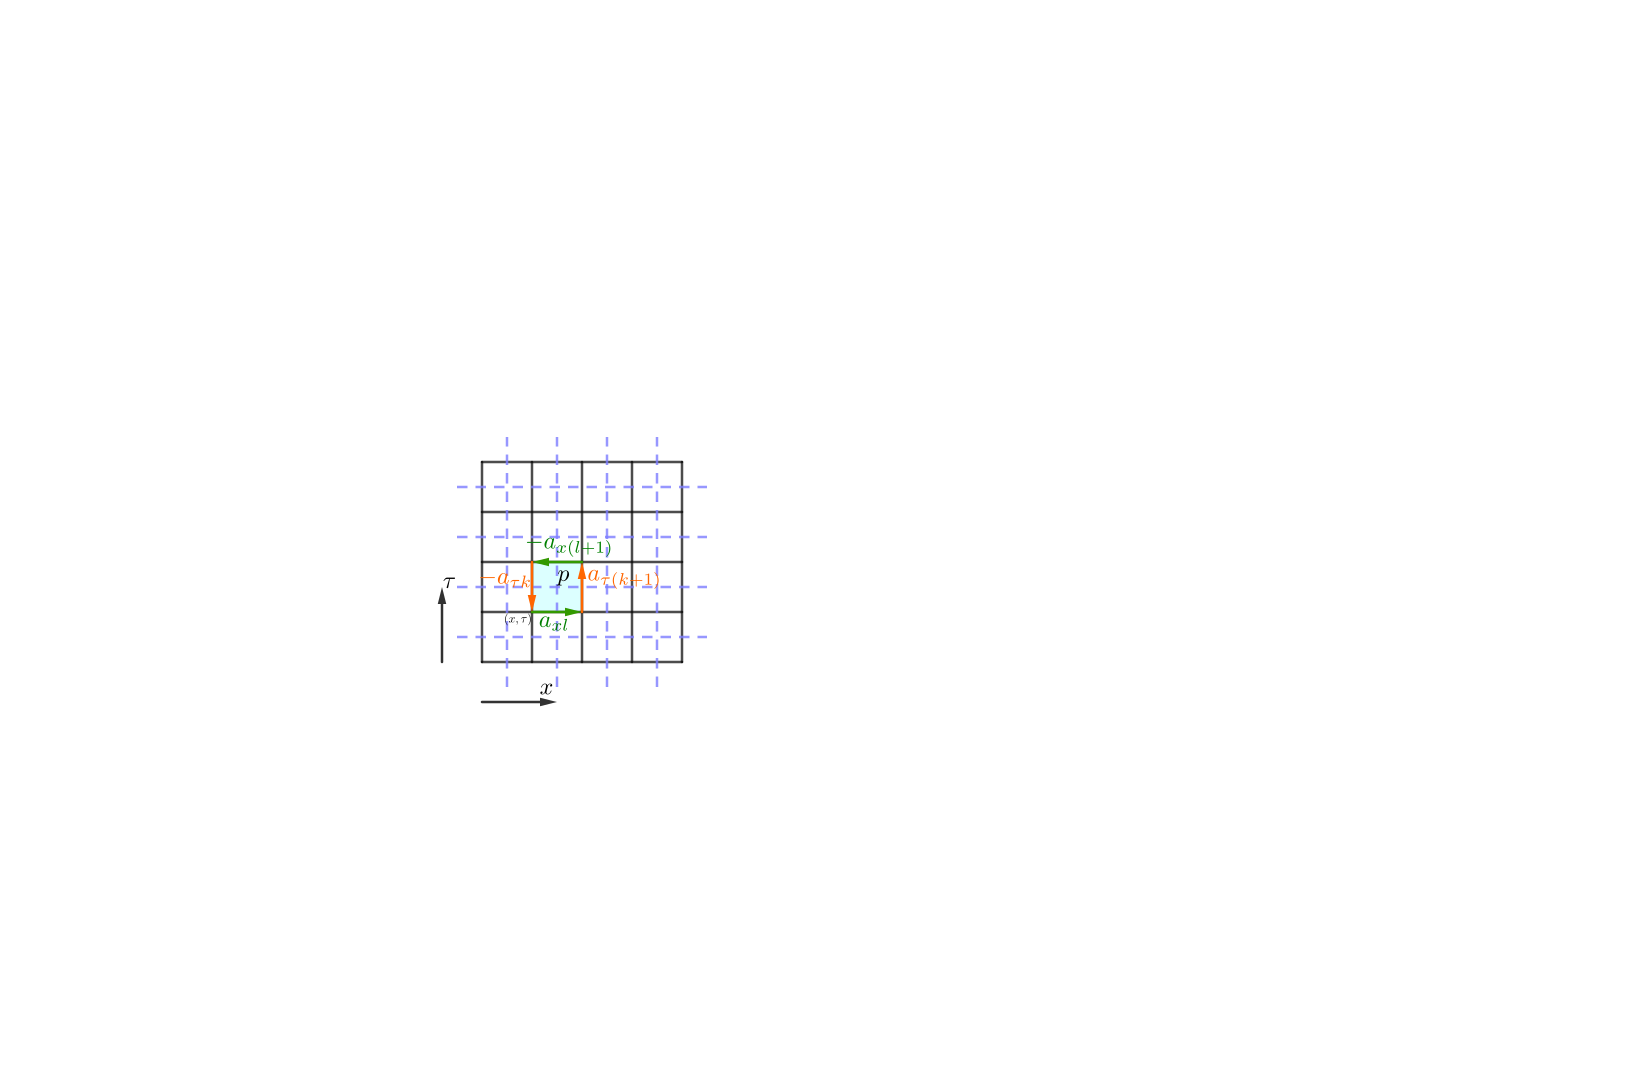
\includegraphics[width = 0.95\linewidth]{lattice.pdf}
    \label{lattice}
\end{wrapfigure}
Perform Wick rotation, $t \rightarrow -i\tau, a_t \rightarrow ia_{\tau}, \partial_t \rightarrow i \partial_{\tau}$, we have 
\begin{equation}
    iS \rightarrow \int {\rm d}\tau {\rm d} x -\frac{1}{2e^2} 
    (\partial_x a_{\tau} - \partial_{\tau} a_x)^2
\end{equation}
To map it to the lattice, we note that $\partial_x a_{\tau} = \frac{a_{\tau}(x+\delta x) - a_{\tau}(x)}{\delta x} \rightarrow \frac{({\rm d}a_{\tau})_p}{\delta x}$, where $ {\rm d}a_\tau \equiv a_{\tau (k+1)} - a_{\tau k} $, we can absorb the distance $\delta x$ in the $x-$direction into the definition of $a_{\tau}$. In the same way, with $\tau-$direction distance $\delta {\tau}$ absorbed by $a_x$, we can define ${\rm d} (a_x)_p \equiv a_{x(l+1)} - a_{xl}$, such that the Lagrangian density is $\mathcal{L} = -\frac{1}{2e^2} ({\rm d}a_{\tau} - {\rm d}a_x)_p^2$. Then the Euclidean lattice path integral is
\begin{equation}
    \mathcal{Z} = (\prod_{x,\tau} \frac{\int {\mathcal{D}} a_{xl} {\mathcal{D}}  a_{\tau k}}{(2\pi)^2})
    \exp \left[\sum_{p} - \frac{1}{2e^2 }
    \left(
        {\rm d}a_{\tau}-{\rm d}a_{x}
    \right)_p^2\right]
\end{equation}
Defining $({\rm d}a)_p \equiv ({\rm d}a_{\tau} - {\rm d}a_x)_p $ and limiting the fields to $(-\pi, \pi)$, we have $ ({\rm d}a)_p\rightarrow ({\rm d}a)_p + 2\pi s_p, s_p \in \mathbb{Z}$, monopoles can be described by $s_p$ and the monopole fugacity term can be written as $\frac{-V}{2} ({\rm d}s)_c^2$. But in (1+1) D spacetime, $({\rm d} s)_c$ does not exist, which means monopoles do not exist.

\begin{wrapfigure}{r}{0.3\linewidth}
    \centering
    \includegraphics[width = 0.8\linewidth]{Two_elections.pdf}
    \label{two_elections}
\end{wrapfigure}
Take the Hubbard-Stratonovich transformation, the Lagrangian density becomes
\begin{equation}
    \mathcal{L} = -\frac{e^2}{2} \pi_p^2 + i\pi_p ({\rm d}a + 2\pi s)_p
\end{equation}
insert Wilson loop representing two charges, which means $w_k = 1$ on the left red line in the above figure, $w_k = -1$ on the right, all the others are zero, and then calculate $\braket{e^{i\sum_k w_k a_{\tau k}}}$. 
By part integration, $\pi _p ({\rm d}a)_p = -(\tilde{\rm d}\tilde{\pi})_{k} a_{\tau k} + (\tilde{\rm d}\tilde{\pi})_{l} a_{x l}$, and integrate out $a_{\tau k}$, we get $(\tilde{\rm d}\tilde{\pi})_{k} = +1$ on the left red line, $(\tilde{\rm d}\tilde{\pi})_{k} = -1$ on the right red line. 
While $k$ corresponding to $l^*$ on the dual lattice, this means $\tilde{\pi} _ {v^*_{red}} - \tilde{\pi}_{v^*_{white}} = 1$. 
Then $\braket{e^{i\sum_k w_k a_{\tau k}}} \propto e^{\sum_p -\frac{e^2}{2} \pi_p^2} \propto e^{-{\rm const.}R}$. So this Euclidean quantum theory always confines as long as $e^2 >0$.

\paragraph{c)}
In this case
\begin{equation}
    \mathcal{Z} = (\prod_{x,\tau, p} \frac{\int_{-\pi}^{\pi} {\mathcal{D}} a_{xl} {\mathcal{D}}  a_{\tau k}}{(2\pi)^2} \sum_{s_p \in \mathbb{Z}})
    \exp \left[\sum_{p} - \frac{1}{2e^2 }
    ({\rm d}a + 2\pi s)_p^2
    + i\frac{\Theta}{2\pi} ({\rm d}a + 2\pi s)_p
    \right]
\end{equation}
$\sum_p ({\rm d}a)_p $ is the total derivative, it could be zero if we choose periodic boundary condition. But $2\pi s_p$ si not a total derivative. Also, when $\Theta \rightarrow \Theta + 2\pi$, the Lagrangian density only changed by adding a term $i 2 \pi s_p$, leaving path integral unchanged.\\
Take the Hubbard-Stratonovich transformation, we have
\begin{equation}
    \mathcal{L} = 
    -\frac{e^2}{2} \pi_p^2 
    + i(\pi_p + \frac{\Theta}{2\pi} )({\rm d}a + 2\pi s)_p
\end{equation}
Using Poisson resummation to sum over $s_p$, we get $\sum_m \delta(\pi_p + \frac{\Theta}{2\pi} - m), m \in \mathbb{Z}$.
In the same way as in $b)$, insert Wilson loop, and by part integration, we have $(\tilde{d} \tilde{\pi})_k = w_k$. So, in the white region, $\pi_p = m - \frac{\Theta}{2\pi}$, while in the red region $\pi_p = m+1 - \frac{\Theta}{2\pi}$.So 
\begin{equation}
    \braket{e^{i\sum_k w_k a_{\tau k}}} 
    = \frac{\sum_m \exp \left[
        - (m - \Theta/2\pi)^2 \cdot {\rm Area_{white}} + (m +1 - \Theta/2\pi)^2 \cdot {\rm Area_{red}}
    \right]}{\sum_m \exp \left[
            - (m - \Theta/2\pi)^2 \cdot ({\rm Area_{white} + \rm Area_{red}})
        \right]}
\end{equation}
Limiting $\Theta \in (0, 2\pi)$, when $\Theta \neq \pi$, the most probable $m = 0 {\rm or} 1$ depending on which makes $m - \Theta /2\pi$ as close to zero as possible, and all the other terms can be neglected as $\rm Area_{white}$ is large enough. In this case, $\braket{e^{i\sum_k w_k a_{\tau k}}}  \propto e^{\rm Area_{red}} = e^{{\rm const.}\cdot R}$, so this theory confines. But when $\Theta = \pi$, $m = 0$. $\braket{e^{i\sum_k w_k a_{\tau k}}} =1$, so this theory de-confines.

\paragraph{d)}
When $\Theta = 0$
\begin{equation}
    \mathcal{Z} = (\prod_{x,\tau, p} \frac{\int_{-\pi}^{\pi} {\mathcal{D}} a_{xl} {\mathcal{D}}  a_{\tau k}}{(2\pi)^2} \sum_{s_p \in \mathbb{Z}})
    \exp \left[\sum_{p} - \frac{1}{2e^2 }
    ({\rm d}a + 2\pi s)_p^2
    \right]
\end{equation}
When $\Theta = \pi$
\begin{equation}
    \mathcal{Z} = (\prod_{x,\tau, p} \frac{\int_{-\pi}^{\pi} {\mathcal{D}} a_{xl} {\mathcal{D}}  a_{\tau k}}{(2\pi)^2} \sum_{s_p \in \mathbb{Z}})
    (-1)^{s_p}\exp \left[\sum_{p} - \frac{1}{2e^2 }
    ({\rm d}a + 2\pi s)_p^2
    \right]
\end{equation}
Both are real. So in these cases theories are time-reversal invariant. To re-interpreted as 2D statistical mechanical system, the path integral must be real and positive. So only $\Theta = 0$ works.

\paragraph{e)}
Villain model coupled to Maxwell theory
\begin{equation}
    \mathcal{L} 
    = - \frac{1}{2e^2 }({\rm d}a + 2\pi s)_p^2
    + i\frac{\Theta}{2\pi} ({\rm d}a + 2\pi s)_p
    + \frac{1}{2T}({\rm d}\theta - a_{x})_l^2 
    + \frac{1}{2T}({\rm d}\theta - a_{\tau})_k^2
\end{equation}
Perform Hubbard-Stratonovich transformation,
\begin{equation}
    \mathcal{L} = 
    -\frac{e^2}{2} \pi_p^2 + i(\pi_p + \frac{\Theta}{2\pi})({\rm d}a+2\pi s)_p
    + \frac{T}{2} J_l^2 + iJ_l ({\rm d}\theta - a)_l 
\end{equation}

After integrating out $a$ by part integration, and sum over $s_p$, we get 
\begin{equation}
    \begin{aligned}
        & (\tilde{\rm d} \tilde{J})_v = 0 \\
        & (\tilde{\rm d} \tilde{\pi})_l + J_l = 0\\
        & \pi_p + \frac{\Theta}{2\pi} \in \mathbb{Z}
    \end{aligned}
\end{equation}

\begin{minipage}{0.3\linewidth}
    \centering
    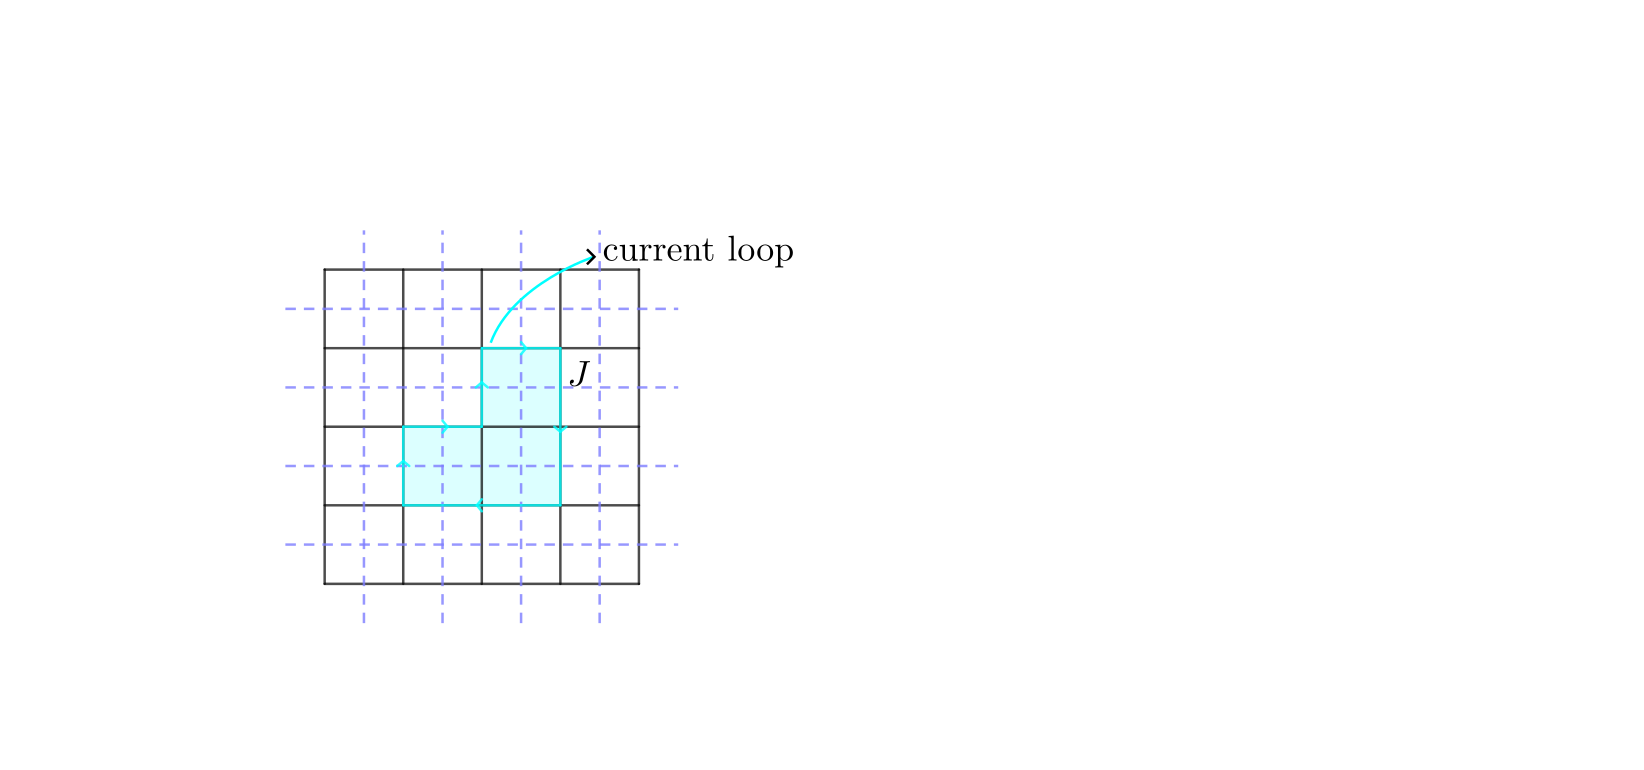
\includegraphics[width = 0.7\linewidth]{EM_matter.pdf}
\end{minipage}
\begin{minipage}{0.3\linewidth}
    \centering
    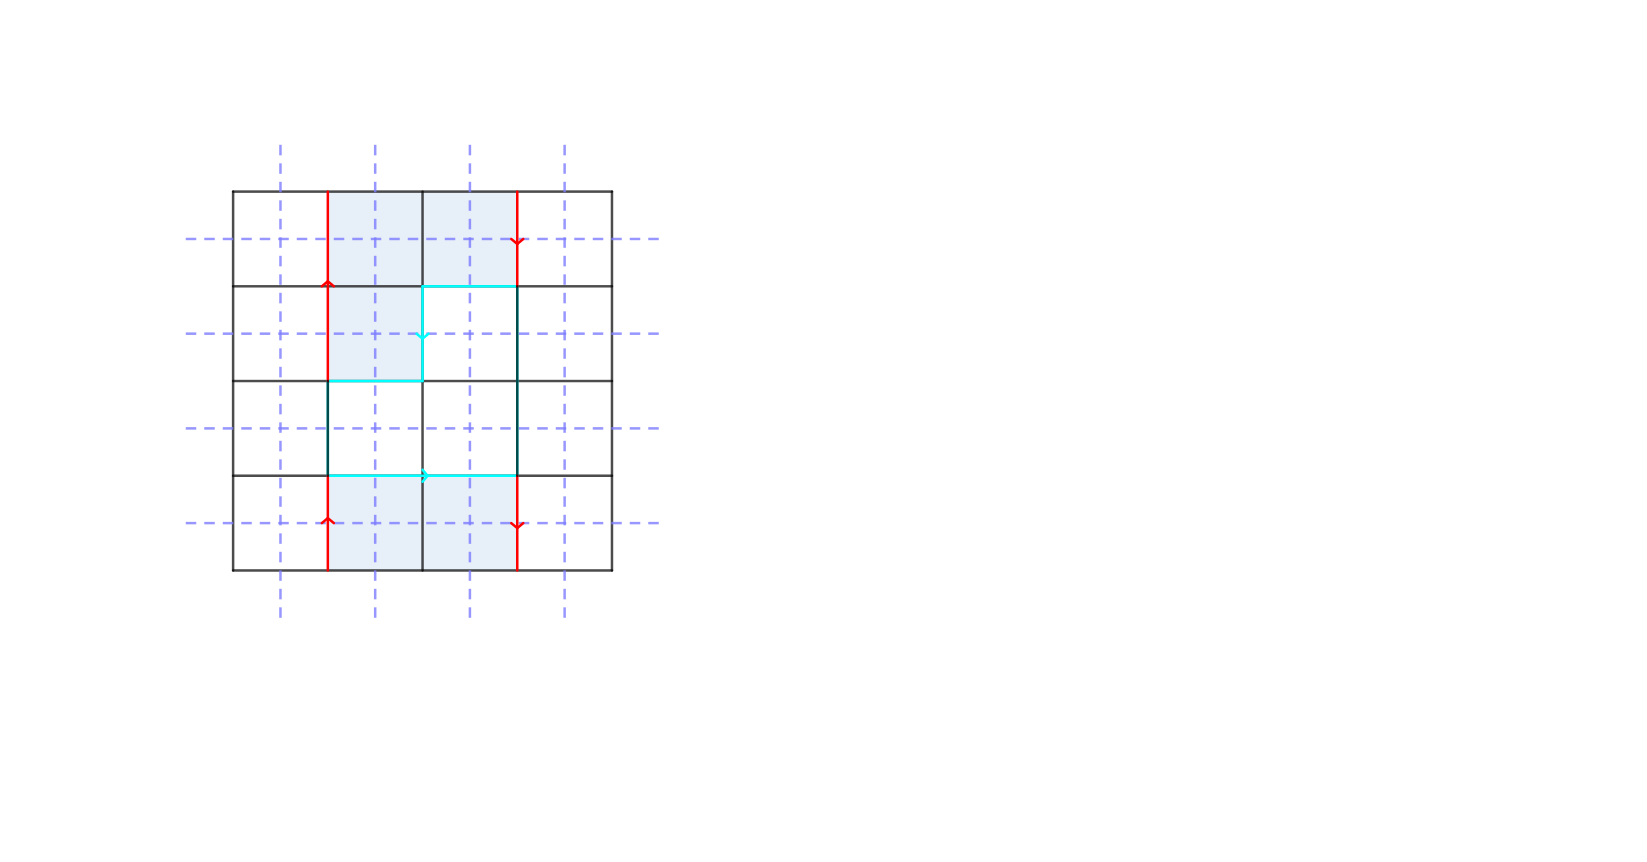
\includegraphics[width = 0.55\linewidth]{EM_matter_wilson.pdf}
\end{minipage}
\begin{minipage}{0.3\linewidth}
    \centering
    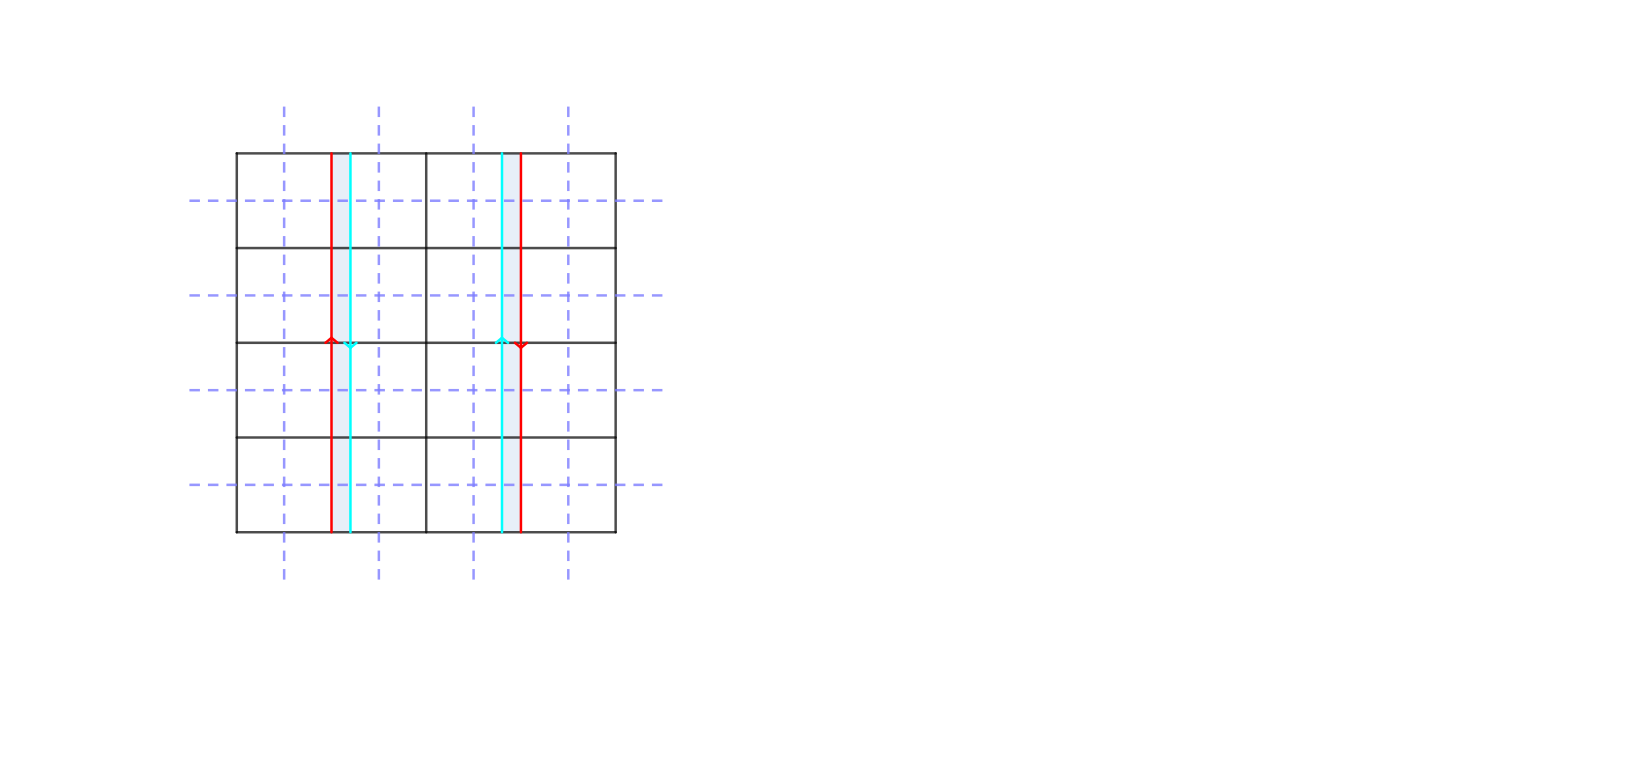
\includegraphics[width = 0.55\linewidth]{screening.pdf}
\end{minipage}

The first equation means current must form loops. The second equation means the $\pi_p$ inside the current loop are different from $\pi_p$ outside the loop by $J$.\\
If we insert Wilson loop and calculate the expectation value, we get $(\tilde{\rm d} \tilde{\pi})_l + J_l = w_l$. So Wilson loop just like current loop with anti-direction. The configuration that current loop minimize the enclosed area together with Wilson loop will dominate the path integral. Which means the current deforms to make the theory does not confine anymore, exactly screening effect.

\paragraph{f)}
Insert two Wilson loops, situation will be different between two phases. When $\Theta = \pi$, when we make charges with the same sign at the same side as illustrated in figure, this theory change to confine. This will not happen to confining $\Theta$ coupled to charged matter.
\begin{figure}
    \centering
    \includegraphics[width = 0.6\linewidth]{two_loop.pdf}
\end{figure}

\end{document}

